\documentclass[14pt]{extbook}
\usepackage{multicol, enumerate, enumitem, hyperref, color, soul, setspace, parskip, fancyhdr} %General Packages
\usepackage{amssymb, amsthm, amsmath, bbm, latexsym, units, mathtools} %Math Packages
\everymath{\displaystyle} %All math in Display Style
% Packages with additional options
\usepackage[headsep=0.5cm,headheight=12pt, left=1 in,right= 1 in,top= 1 in,bottom= 1 in]{geometry}
\usepackage[usenames,dvipsnames]{xcolor}
\usepackage{dashrule}  % Package to use the command below to create lines between items
\newcommand{\litem}[1]{\item#1\hspace*{-1cm}\rule{\textwidth}{0.4pt}}
\pagestyle{fancy}
\lhead{Progress Quiz 4}
\chead{}
\rhead{Version B}
\lfoot{4378-7085}
\cfoot{}
\rfoot{Fall 2020}
\begin{document}

\begin{enumerate}
\litem{
Choose the equation of the function graphed below.
\begin{center}
    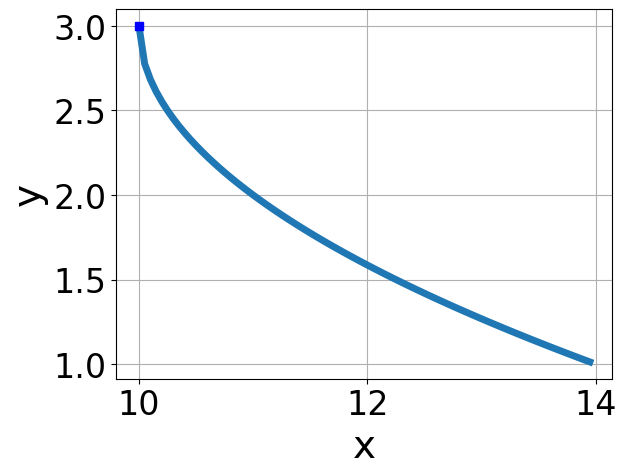
\includegraphics[width=0.5\textwidth]{../Figures/radicalGraphToEquationB.png}
\end{center}
\begin{enumerate}[label=\Alph*.]
\item \( f(x) = - \sqrt[3]{x - 12} - 4 \)
\item \( f(x) = - \sqrt[3]{x + 12} - 4 \)
\item \( f(x) = \sqrt[3]{x - 12} - 4 \)
\item \( f(x) = \sqrt[3]{x + 12} - 4 \)
\item \( \text{None of the above} \)

\end{enumerate} }
\litem{
Solve the radical equation below. Then, choose the interval(s) that the solution(s) belongs to.\[ \sqrt{-10 x^2 + 20} - \sqrt{17 x} = 0 \]\begin{enumerate}[label=\Alph*.]
\item \( x \in [-1.2,3.8] \)
\item \( x \in [-5.5,0.5] \)
\item \( x_1 \in [-5.5, 0.5] \text{ and } x_2 \in [-2.2,1.8] \)
\item \( x_1 \in [-1.2, 3.8] \text{ and } x_2 \in [2.5,11.5] \)
\item \( \text{All solutions lead to invalid or complex values in the equation.} \)

\end{enumerate} }
\litem{
What is the domain of the function below?\[ f(x) = \sqrt[7]{-7 x + 9} \]\begin{enumerate}[label=\Alph*.]
\item \( \text{The domain is } (-\infty, a], \text{   where } a \in [1.2, 2.4] \)
\item \( (-\infty, \infty) \)
\item \( \text{The domain is } [a, \infty), \text{   where } a \in [1.17, 1.3] \)
\item \( \text{The domain is } [a, \infty), \text{   where } a \in [0.28, 0.9] \)
\item \( \text{The domain is } (-\infty, a], \text{   where } a \in [0.7, 1.1] \)

\end{enumerate} }
\litem{
Solve the radical equation below. Then, choose the interval(s) that the solution(s) belongs to.\[ \sqrt{6 x - 5} - \sqrt{-6 x - 3} = 0 \]\begin{enumerate}[label=\Alph*.]
\item \( x_1 \in [-0.29, 0.36] \text{ and } x_2 \in [-1.17,1.83] \)
\item \( x \in [-0.29,0.36] \)
\item \( \text{All solutions lead to invalid or complex values in the equation.} \)
\item \( x_1 \in [-0.89, -0.02] \text{ and } x_2 \in [-1.17,1.83] \)
\item \( x \in [0.44,0.82] \)

\end{enumerate} }
\litem{
Choose the graph of the equation below.\[ f(x) = \sqrt{x + 8} + 6 \]\begin{enumerate}[label=\Alph*.]
\begin{multicols}{2}\item 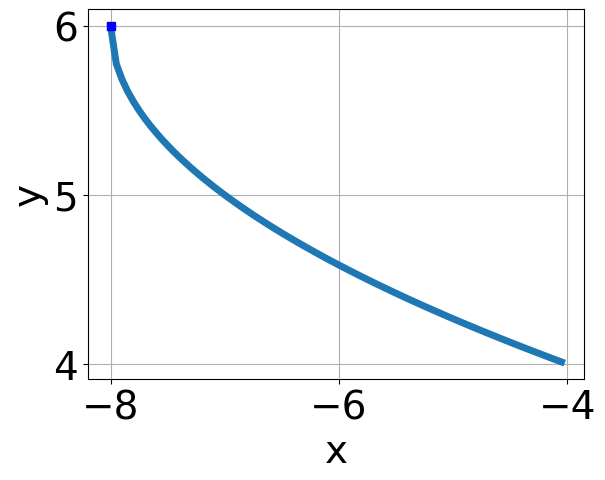
\includegraphics[width = 0.3\textwidth]{../Figures/radicalEquationToGraphCopyAB.png}\item 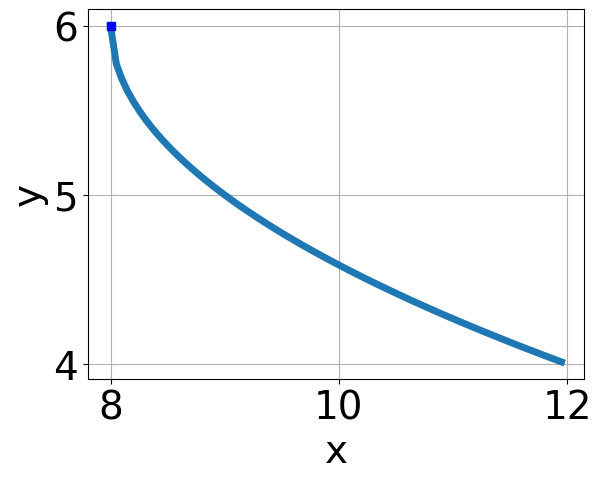
\includegraphics[width = 0.3\textwidth]{../Figures/radicalEquationToGraphCopyBB.png}\item 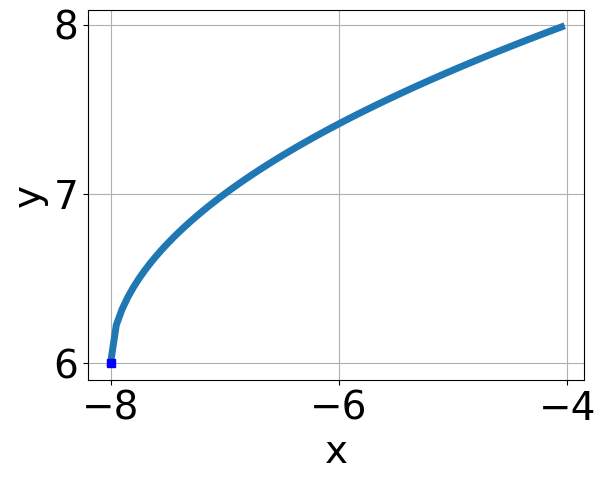
\includegraphics[width = 0.3\textwidth]{../Figures/radicalEquationToGraphCopyCB.png}\item 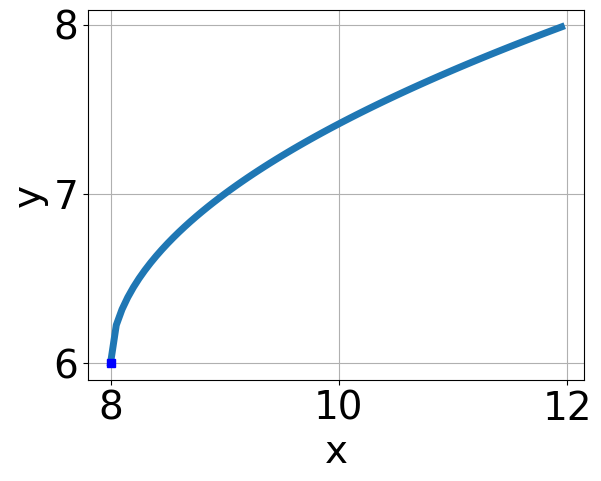
\includegraphics[width = 0.3\textwidth]{../Figures/radicalEquationToGraphCopyDB.png}\end{multicols}\item None of the above.
\end{enumerate} }
\litem{
Choose the graph of the equation below.\[ f(x) = \sqrt{x - 12} - 6 \]\begin{enumerate}[label=\Alph*.]
\begin{multicols}{2}\item 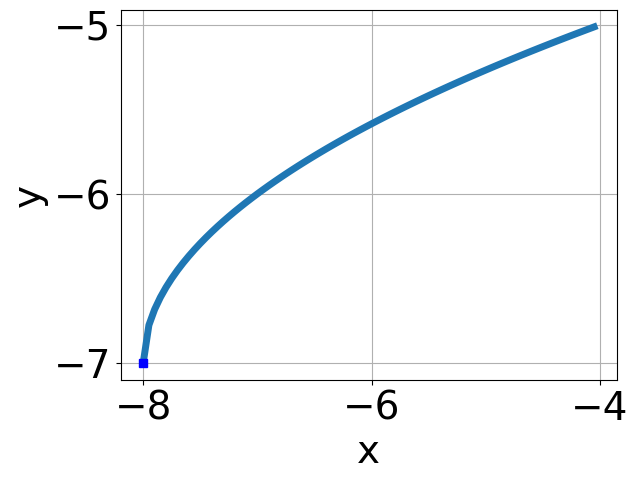
\includegraphics[width = 0.3\textwidth]{../Figures/radicalEquationToGraphAB.png}\item 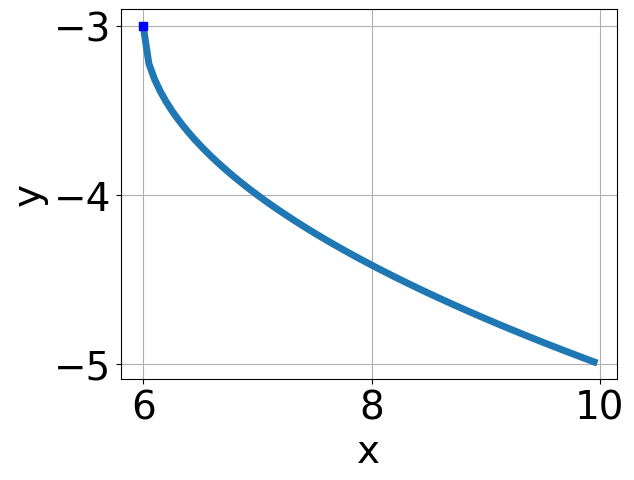
\includegraphics[width = 0.3\textwidth]{../Figures/radicalEquationToGraphBB.png}\item 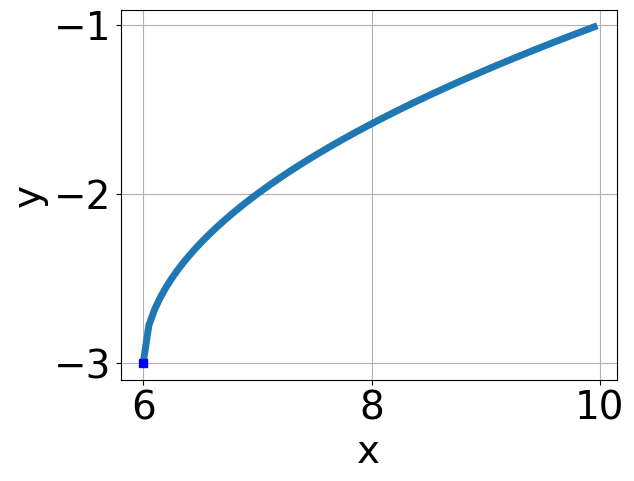
\includegraphics[width = 0.3\textwidth]{../Figures/radicalEquationToGraphCB.png}\item 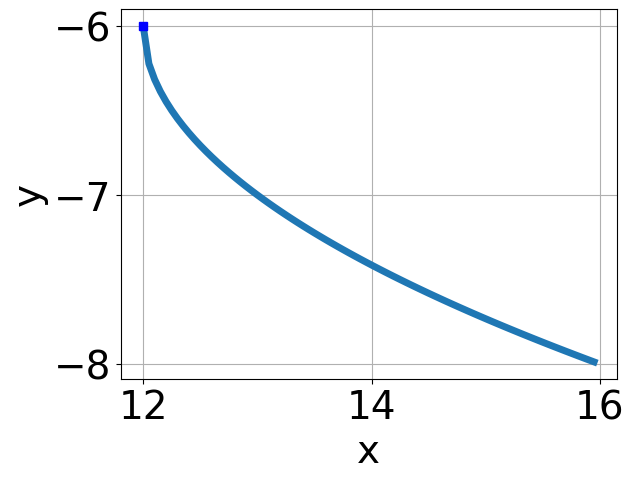
\includegraphics[width = 0.3\textwidth]{../Figures/radicalEquationToGraphDB.png}\end{multicols}\item None of the above.
\end{enumerate} }
\litem{
Choose the equation of the function graphed below.
\begin{center}
    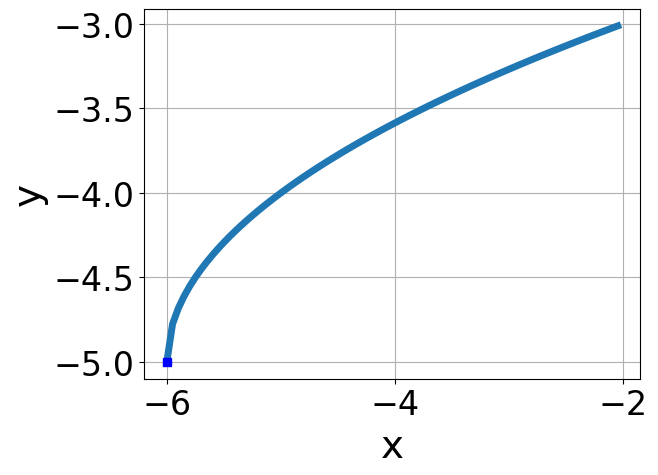
\includegraphics[width=0.5\textwidth]{../Figures/radicalGraphToEquationCopyB.png}
\end{center}
\begin{enumerate}[label=\Alph*.]
\item \( f(x) = \sqrt[3]{x - 6} - 6 \)
\item \( f(x) = \sqrt[3]{x + 6} - 6 \)
\item \( f(x) = - \sqrt[3]{x - 6} - 6 \)
\item \( f(x) = - \sqrt[3]{x + 6} - 6 \)
\item \( \text{None of the above} \)

\end{enumerate} }
\litem{
What is the domain of the function below?\[ f(x) = \sqrt[4]{-4 x - 9} \]\begin{enumerate}[label=\Alph*.]
\item \( [a, \infty), \text{where } a \in [-0.7, 0.9] \)
\item \( (-\infty, \infty) \)
\item \( (-\infty, a], \text{ where } a \in [-3, -2.1] \)
\item \( (-\infty, a], \text{where } a \in [-1, 1.2] \)
\item \( [a, \infty), \text{where } a \in [-2.8, -0.9] \)

\end{enumerate} }
\litem{
Solve the radical equation below. Then, choose the interval(s) that the solution(s) belongs to.\[ \sqrt{27 x^2 + 63} - \sqrt{90 x} = 0 \]\begin{enumerate}[label=\Alph*.]
\item \( x \in [1.3,3.1] \)
\item \( x \in [-1.3,1.1] \)
\item \( x_1 \in [-1.3, 1.1] \text{ and } x_2 \in [1.33,3.33] \)
\item \( \text{All solutions lead to invalid or complex values in the equation.} \)
\item \( x_1 \in [-4.8, 0.1] \text{ and } x_2 \in [-2,0] \)

\end{enumerate} }
\litem{
Solve the radical equation below. Then, choose the interval(s) that the solution(s) belongs to.\[ \sqrt{-5 x + 8} - \sqrt{4 x - 6} = 0 \]\begin{enumerate}[label=\Alph*.]
\item \( x_1 \in [1.54, 1.58] \text{ and } x_2 \in [0.6,5.6] \)
\item \( x_1 \in [1.45, 1.5] \text{ and } x_2 \in [0.6,5.6] \)
\item \( x \in [0.14,0.33] \)
\item \( \text{All solutions lead to invalid or complex values in the equation.} \)
\item \( x \in [1.54,1.58] \)

\end{enumerate} }
\end{enumerate}

\end{document}